\documentclass[12pt,a4paper,notitlepage]{article}
%%%%%%%%%%%%%%%%%%%%%%%%%%%%%%%%%%%%%%%%%%%%%%%%%%%%%%%%%%%%%%%%%%%%%
% Template pour rendus Master
%%%%%%%%%%%%%%%%%%%%%%%%%%%%%%%%%%%%%%%%%%%%%%%%%%%%%%%%%%%%%%%%%%%%%%
%\documentclass[12pt,a4paper,titlepage]{report}
\usepackage[utf8]{inputenc} %encodage
\usepackage[square,sort,comma,numbers]{natbib} % bibliography
\setcitestyle{authoryear,open={(},close={)}}
\renewcommand{\bibsection}{}

\usepackage[french]{babel} % langue

%mise en page générale
\usepackage{geometry}
%\geometry{a4paper} % format de feuille
\geometry{top=2.5cm, bottom=2.5cm, left=2.5cm, right=2.5cm} %marges
%Police
\usepackage{mathptmx} % Times si compilateur pdfLatex
%interligne
\linespread{1.5}
%en tete et pied de page
\usepackage{fancyhdr}
\usepackage{lastpage}
\pagestyle{plain}

\usepackage{hyperref} % lien cliquables
\usepackage{url, lipsum} %Lorem ipsum

\usepackage{wrapfig} %position d'images dans le texte
%\usepackage[myheadings]{fullpage}
\usepackage{graphicx, subcaption, setspace, booktabs}

\usepackage[table]{xcolor}

\usepackage{caption}
\DeclareCaptionType{annexe}[Annexe][Liste d'annexes] % rajout pour mettre des captions annexes

\DeclareCaptionType{web}[Web][Sites Web] % rajout pour mettre des captions web

\usepackage{lscape}

\usepackage{subcaption}

\usepackage{todonotes}

\usepackage[export]{adjustbox}

\DeclareRobustCommand{\rchi}{{\mathpalette\irchi\relax}}
\newcommand{\irchi}[2]{\raisebox{\depth}{$#1\chi$}}

%%%%%%%%%%%%%%%%%%%%%%%%%%%%%%%%%%%%%%%%%%%%%%%%%%%%%%%%%%%%%%%%%%%%%%
% Page de garde et table des matières
%%%%%%%%%%%%%%%%%%%%%%%%%%%%%%%%%%%%%%%%%%%%%%%%%%%%%%%%%%%%%%%%%%%%%%
\title{\textbf{Délimitation d'espèces au sein du complexe de plantes des Alpes, \textit{Primula pedemontana s.l.}}}
\author{Maxime Jaunatre, Master 1 BEE Grenoble}
\date{1 Avril - 31 Mai 2019  |  Soutenance : juin 2019 }

\renewcommand*\contentsname{Table des matières}

\begin{document}

\begin{titlepage} %Page de garde!!
%logos de page de garde
\begin{figure}
  \centering
\begin{subfigure}{0.4\textwidth}
  %\centering
  
\includegraphics[width=0.7\linewidth,left]{fig/UGA.jpg}
\end{subfigure}%
\begin{subfigure}{.4\textwidth}
  %\centering
  
\includegraphics[width=0.7\linewidth,right]{fig/leca.jpg}
\end{subfigure}
\label{fig:test}
\end{figure}
%titres
\maketitle


\noindent
\begin{minipage}{1.3in}
\textbf{\underline{Enseignant référent:}} \\
Éric Coissac
\end{minipage}
\hfill
\begin{minipage}{1.3in}
\textbf{\underline{Tuteur de stage:}} \\
Florian Boucher
\end{minipage}
\hfill
\begin{minipage}{1.3in}
\textbf{\underline{Équipe:}} \\
DivAdapt
\end{minipage}

%image sympas
\begin{figure}[h]
\begin{center}
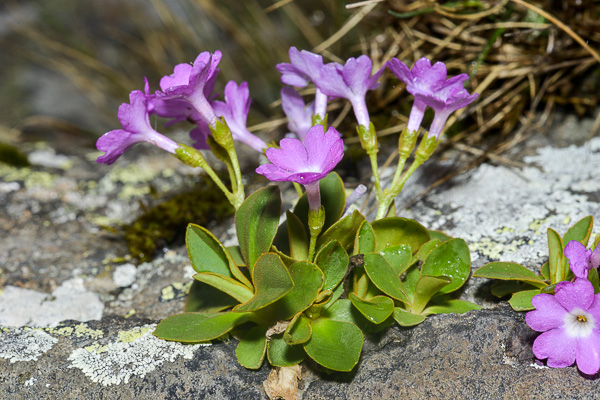
\includegraphics[scale=3]{fig/primulapedemontana_7.jpg}
%	\caption{reference de la photo}
%	\label{frontpage}

\end{center}
\end{figure}
\thispagestyle{empty}

{\let\thefootnote\relax\footnote{{ \textit{Primula pedemontana} Crédit photo : Florian Boucher}}}

\newpage
\begin{abstract} %abstract!!!
\begin{center}

\lipsum[1]

\end{center}
\end{abstract}
\thispagestyle{empty}

\end{titlepage}
\tableofcontents

\newpage
%%%%%%%%%%%%%%%%%%%%%%%%%%%%%%%%%%%%%%%%%%%%%%%%%%%%%%%%%%%%%%%%%%%%%%
% BODY
%%%%%%%%%%%%%%%%%%%%%%%%%%%%%%%%%%%%%%%%%%%%%%%%%%%%%%%%%%%%%%%%%%%%%%
%Consignes pour rapport et soutenance du stage M1

%Le rapport
%Il doit comporter 12 pages (+/1page) figures comprises, sommaire et références biblio en plus, annexes déconseillées. Moins de 20 références bibliographiques, 12 lignes de résumé au dos de la couverture.
%Le plan à adopter a priori est « Introduction / Matériel et méthodes / Résultats / Discussion » à moins qu’il ne soit pas adapté à votre travail (c’est rarement le cas).
%Format : TIMES 12 points, avec un interligne 1,5. Le rapport peut être rédigé en Français ou en Anglais.
%Les personnes qui font un stage long et concentrent leur rapport sur la mise au point de la méthodologie (c'est à dire n'ayant pas de résultats au moment de la soutenance) sont encouragées à expliquer ce contexte dans un court préambule d'une dizaine de lignes maximum. Les membres de jury sont informés de l'éventualité d'une telle situation.
%Le rapport de stage est à rendre à votre responsable pédagogique de stage pour le :
%Mardi 28 mai 2018 à 12 h au plus tard
%Une version papier adressée par courrier ou déposée au secrétariat du LECA. Une version pdf envoyée par mail au tuteur de stage et au responsable du M1.
%L’envoi uniquement au format électronique peut se faire à titre exceptionnel (stage à l’étranger nécessitant un long délai d’acheminement – contacter par email votre responsable pédagogique avant).

%La soutenance
%Modalités : 10 min de présentation + 5 min de questions devant un jury de 3 personnes. Le maître de stage est invité à venir écouter la soutenance s’il le souhaite.
%Format de présentation : fichier pdf ou ppt sur clé USB. Les soutenances auront lieu la semaine du 3 Juin 2019. Un planning de soutenance vous sera communiqué fin mai. Les étudiants effectuant un stage long à l’étranger et ne rentrant pas en France peuvent soutenir par visioconférence.
%Contacter votre responsable pédagogique par email mi mai pour fixer les modalités.

%Fiche d’évaluation
%La fiche d'évaluation doit être donnée à votre encadrant en début de stage. Elle sera renvoyée par email par le maître de stage au plus tard le 1 er juin 2019.
%Attention : pour les stages longs à l'étranger prévoyez l'éventualité d'un retour à Grenoble en cas de rattrapage (seconde session d'examen deuxième quinzaine de juin première quinzaine de juillet).
\section{Introduction}

\lipsum[1-2]
\todo{Don't forget to put a real introduction here.}
%

%%%%% intro de flo %%%%%%

%Déterminer quelles entités taxonomiques constituent des espèces distinctes est un des objectifs premier de la taxonomie mais est également d’une importance primordiale pour comprendre à la fois l’origine des espèces, le processus de spéciation, et leur futur probable, qui détermine les mesures de conservation qui sont éventuellement à prendre pour les protéger.
%	Si délimiter des espèces vivant en sympatrie est généralement une tâche facile, les complexes d’espèces cryptiques ayant des distributions allopatriques présentent souvent plus de difficulté (Coyne & Orr 2004). En effet, dans ces derniers cas les critères qui servent généralement à établir la présence d’isolement reproductif (absence de flux de gènes ou  d’individus hybrides entre lignées, etc.) ne peuvent pas être mesurés objectivement (Fujita et al. 2012). Pourtant, délimiter des espèces cryptiques distribuées en allopatrie permet d’étudier le rôle d’un des mécanismes de spéciation majeurs : l’isolement géographique (Mayr 1942). Dans certains cas où la dynamique de l’environnement abiotique au cours du temps est bien connue, de telles études permettent même de caractériser précisément l’influence de l’environnement sur la divergence évolutive entre lignées (Avise et al. 1987).

%	Dans le cadre de ce stage, nous tenterons de comprendre comment la dynamique du relief dans les Alpes (i.e. les phénomènes d’orogénèse, d’érosion et de glaciation) a contribué à la divergence d’espèces au sein d’un groupe de plantes de haute montagne : Primula sect. Auricula Scott subsect. Erythrodrosum Pax (ci-dessous, clade Hirsuta). Ce groupe comprend traditionnellement six espèces proches de P. hirsuta All. mais une étude récente a proposé de re-circonscrire P. pedemontana en fusionnant trois espèces, tout en suggérant qu’un taxon distinct existe dans le massif des Ecrins en France (Boucher et al. 2016). Nos objectifs de recherche seront les suivants :
%	1) Reconstruire les relations phylogénétiques entre taxons du clade Hirsuta et dater leurs divergences
%	2) Délimiter les taxons qui méritent le rang d’espèce au sein de ce clade et en particulier au sein du complexe de P. pedemontana s.l.
%	3) Comparer statistiquement différents scénarios afin de comprendre comment la dynamique des reliefs Alpins a influencé la divergence des espèces du clade Hirsuta

%	Pour cela, nous utiliserons des données de séquençage haut-débit obtenues grâce à la technique hyRAD (Suchan et al. 2016) . Ces données comprennent plusieurs milliers de SNPs indépendants pour 22 individus appartenant aux six espèces du clade Hirsuta actuellement reconnues (Boucher et al. 2016). Nous les analyserons d’abord avec des approches phylogénétiques standard comme le logiciel RAxML (Stamatakis 2014) et des avancées nouvelles permettant de dater des phylogénies inférées grâce à des SNPs (Stange et al. 2018). Afin de délimiter des espèces le plus objectivement possible à l’aide des données moléculaires disponibles, nous utiliserons la panoplie variée des techniques de la taxonomie moléculaire, incluant des techniques de clustering génétique mais aussi d’autre basées sur le coalescent (Fujita et al. 2012, Carstens et al. 2013, Leaché et al. 2014). Enfin, nous aurons recours à l’inférence ABC pour comparer explicitement différents scénarios de spéciation (Knwoles 2009, Cornuet et al. 2014).

%	Cette étude devrait nous aider à mieux comprendre l’influence de la dynamique du relief sur l’évolution de la flore des Alpes. Elle permettra également d’établir plus fermement le statut taxonomique du nouveau taxon de Primula découvert dans le massif des Ecrins, qui reste à ce jour un mystère (http://www.ecrins-parcnational.fr/actualite/lenigme-de-la-primevere-du-valgaudemar), et éventuellement d’envisager des mesures de conservation.



\section{Matériels et méthodes}

\subsection{Échantillonnage}

Les données génétiques utilisés lors de cette étude ont été produite dans le cadre de l'étude précédente de \citet{Boucher2016a}. 
Il s'agit d'un jeu de donnée composé de 90 individus des espèces composant la section \textit{Auricula}, au sein du genre \textit{Primula}. 
Ces individus ont été prélevés à travers les Alpes entre avril et septembre 2014. 
L'identification taxonomique des individus a été réalisé sur le terrain, mais un individu a du être réattribué après analyse génétique au taxon \textit{P. hirsuta}.

Les SNPs sont issus de séquençage haut débit via hyRAD \citep{Suchan2016}. 
Le génome de référence proviens de \textit{Primula veris}.
Cette technique permet de génotyper le long du génome malgré des mutations sur les sites de restrictions. 
En effet les enzymes de restrictions sont trop sensibles à la mutation d'un nucléotide, tandis que les sondes ARN peuvent s'hybrider sur des sites plus nombreux sur le génome. 
La nécessité de capturer des sites malgré une faible variation provient du niveau interspécifique de l'étude, qui pose l'hypothèse que les mutations peuvent se placer sur les sites de restrictions et ainsi limiter leur capture par simple séquençage ddRAD.
% extrait d'article de base :
%Total DNA was extracted from silica-dried leaves using a DNeasy Plant Mini kit (Qiagen, Hilden, Germany) following the manufacturer’s instructions. DNA quality was visualized on 0.8% agarose gels and quantity was assessed using a QuBit 2.0 fluorom- eter (2.0, Life Technologies, Carlsbad, CA, USA). Genomic DNA was converted into RAD-Capture genotyping-by-sequencing libraries (SNPsaurus, LLC), a new protocol aimed at harnessing the wide genomic spectrum of RAD-sequencing while reducing the amount of missing data in interspecific datasets. Briefly, a double-digest RAD library was created from 100 ng of a pool of genomic DNA containing a diverse set of individuals from sect. Auricula (belong- ing to P. allionii, P. apennina, P. auricula, P. glutinosa, and P. minima; see Table A.1). The pooled DNA was digested with PstI-HF and MfeI- HF (NEB) and ligated to complementary adapters that allowed the resulting amplified fragments to be converted to biotinylated RNA baits. Fragments with inserts roughly 100–350 bp in size were iso- lated by gel extraction from a portion of the ligated product prior to amplification and the in vitro transcription reaction to create the RNA baits. Shotgun sequencing libraries were prepared from the 90 study samples using 5 ng each in a 1/10th Nextera (Illumina, Inc) reaction with unique dual-indexes to distinguish the individu- als. The samples were pooled and size-selected for insert sizes roughly 170–370 bp. The pooled libraries were then used in two successive overnight hybridizations to the biotinylated bait library, followed by capture using DynabeadsÒ MyOneTM Streptavidin C1 magnetic beads (Thermo Fisher) and amplification. The final cap- tured products were sequenced in a single 150 bp NextSeq 500 High Output run at the Genomics and Cell Characterization Core of the University of Oregon.

\subsection{Bioinformatique}

Pour chacun des individus, l'information consiste en une séquence de SNPs appellés par Freebayes, exporté sous format VCF. 
Les analyses ont été porté sur deux jeux de données car filtrés sous des seuils différents.
Le premier jeu de donnée ('\verb|m30_-q20_mincov20|') est issus de filtres très strict, avec un score de qualité (Phred) requis de 30 et une couverture minimale de 20 lectures par site. 
Afin de ne pas biaiser l'analyse par des seuils favorisant les régions conservées, le second jeu de données ('\verb|m13_-q20_mincov10|') est quant à lui produit avec un Phred minimal de 13 et une couverture de 10 lectures. 
A partir de ces séquences, les SNPs ont été isolés par Freebayes, avec un score de Phred minimal de 20 et un support de lecture de 30\% minimum par allèle.

A partir des deux jeux de donnée initiaux, un pipeline est établis pour générer divers ensembles de données. 
Cette automatisation a permis de générer les jeux de données spécifiques à chaque analyse. 
Les fonctions sont rassemblées en un package R hébergé sur Github (lien web \ref{github})
Dans un premier temps, le fichier initial est traité sous Rstudio \citep{RTeam2017}, avec la fonction \verb|subset_reorder|, qui permet de reconstruire le fichier en ne gardant que les individus souhaité dans l'ordre indiqué. 
Au maximum, les individus conservés à partir des jeux de données initiaux sont les individus des espèces suivantes :
2 individus de \textit{P. apennina}, 
3 individus de \textit{P. cottia}, 
2 individus de \textit{P. pedemontana}, 
2 individus de \textit{P. pedemontana} des Écrins, 
6 individus de \textit{P. hirsuta}, 
4 individus de \textit{P. villosa}, 
2 individus de \textit{P. daonensis}.
Un individu de \textit{P. apennina} n'a pas été conservé comme dans l'étude de \citet{Boucher2016a}, car présentant trop de données manquantes.
Toutes les informations concernant les individus de l'analyse sont présentés en annexe \ref{table_ind}.


La fonction suivante \verb|rare|, permet de trier les allèles considérés comme étant présents dans un trop faible pourcentage des individus. 
Ces allèles rares sont écartés du jeu de donnée et le loci pour l'individu présentant cet allèle rare est considéré comme une donnée manquante. 
Cette étape permet également de supprimer les lectures avec de multiples allèles variants qui sont reconnus comme des artefacts des algorithmes utilisés pour appeler les SNP.  
%We then filtered variants in a very conservative way by removing all called multiple nucleotide polymorphisms, indels and complex variants. These types of variants are known to often be artifacts generated by the algorithms used for short read mapping (see https://www. broadinstitute.org/gatk/guide/best-practices.php).
Suite aux deux tris précédents, il y a donc des loci pour lesquels tout les individus portent la même information. 
Afin de ne garder que les loci polymorphiques, une fonction \verb|clean| est donc appelée à la fin de la fonction \verb|rare|, pour supprimer les locis monomorphiques.
Les loci sont aussi filtré sur le score de qualité (\verb|QUAL|) indiqué dans le vcf, qui correspond a la confiance dans l'assignation de l'allèle variant. 
%In the context of variant calling, Phred-scaled quality scores can be used to represent many types of probabilities. The most commonly used in GATK is the QUAL score, or variant quality score. It is used in much the same way as the base quality score: the variant quality score is a Phred-scaled estimate of how confident we are that the variant caller correctly identified that a given genome position displays variation in at least one sample
Une fonction de \verb|tri| est appelé pour supprimer les loci puis individus présentant trop de données manquantes selon les seuils posés.
Enfin, afin de limiter le déséquilibre de liaisons, les sites sont filtrés selon leurs positions sur les contigs, où une distance minimale \verb|n| doit être prise en compte entre deux sites d'un même contig pour que le second site soit conservé.


Afin de pouvoir utiliser les fichiers triés sous divers format, la sous-sélection d'individus et de loci est enregistrée sous quatre formats : \verb|.vcf|, \verb|.str|, \verb|.geno|, \verb|.snp|. 
La transformation d'un format en un autre se fait respectivement au moyen d'un script bash, par l'utilisation du software PGDSpider \citep{Lischer2012}, le package LEA \citep{Frichot2015} et un script R. 
La production de ces fichiers est inscrite dans le pipeline par la fonction \verb|files|.

L'ensemble de ces fonctions sont indépendantes mais peuvent être appelées dans le bon ordre au moyen de la fonction \verb|dataset|, qui prend en entrée un vecteur de noms d'individus, un \verb|csv| contenant les assignations aux populations, le fichier \verb|vcf| original, le nom des fichiers de sortie et les seuils précisés au-dessus.


Chaque seuil est choisis après vérification que la décision n'impacte que peu les résultats de diversité génétique.
Le nombre d'individus étant faible, il faut optimiser le nombre de SNPs par individus car cela permet de limiter la perte d'information et d'atteindre les mêmes résultats qu'attendus avec un échantillon plus vaste. \citep{Nazareno2017}


\subsection{Génétique des populations}

Les analyses de génétique des populations ont été réalisés sous Rstudio \citep{RTeam2017} avec différents packages. 

Dans un premier temps, des statistiques F sont calculées avec le package adegenet \citep{Jombart2011}. Ces statistiques permettent de se faire une première idée du jeu de donnée.
Ce package permet également de réaliser un analyse en composante principale discriminante.
Cependant un clustering de nos individus a été réalisé avant, afin d'essayer d'attribuer des groupes sans a-priori de populations.
Ce clustering fait par adegenet trouve les groupes pour lesquels la variance intergroupes est maximale quand la variance intragroupes est minimale.
La DAPC a donc été réalisée avec ces groupes et sans afin d'observer les différences.

La structure des populations de nos taxons a ensuite été étudié par le package LEA \citep{Frichot2015}.
Ce package permet une implémentation dans R des analyses auparavant menées par le logiciel STRUCTURE.
Pour cette étude, la structuration a été modélisée pour des structure de K populations allant de 1 à 15, avec 20 simulations par K, en ne retenant que la meilleurs simulation basée sur le critère de "cross-entropy".
Une dernière mesure de génétique des populations a été réalisé pour essayer d'estimer l'expension ou la contraction récente des populations. Ce \verb|D| de Tajima est mesuré à l'aide du package pegas \citep{Paradis2010}.

Concernant l'hypothèse d'hybridation pour le taxon des Écrins, le package introgress \citep{Gompert2010} a été utilisé pour mesurer l'index h, index d'hybridation, entre deux taxons.
Ce package requiert l'import des deux taxons parents présumés et des hybrides afin de mesurer un coefficient d'admixture (ou h-index).
Ce coefficient basé sur une fonction de vraisemblance \citep{Buerkle2005}, où la proportion de chaque génome parental est mesurée dans l'individu hybride.
Les marqueurs codominants utilisés ici n'étant pas fixés, le calcul du h-index se basera ici sur les fréquences alléliques.
\todo{To do}

\subsection{Inférences bayesiennes}

Afin de caractériser l'admixture probable entre le taxon des Écrins et \textit{P. hirsuta}, une approche par approximate Bayesian computation (ABC) a été réalisée sur le logiciel DIYABC \citep{Cornuet2014}. 
Ce logiciel permet de simuler des jeux de données selon divers scénarios, en échantillonnant des paramètres entre des priors définis. 
Les scénarios sont ensuite classés selon les probabilités a posteriori d'observer notre jeu de donnée initial selon les scénarios proposés. 
Seuls quelques scénarios ont été étudiés ici, en prenant en compte le fait qu'ils sont à chaque fois supportés par peu d'individus. 
Les priors sont également proposés dans un grand intervalle et selon une distribution uniforme, les temps de divergence entre populations et taille de population n'ayant pas été étudiés sur le terrain.

Pour les topologies proposés en scénarios, toutes les topologies "classiques" avec aucun événement d'hybridation sont essayées ( 5 cas possibles pour les 4 taxons \textit{hirsuta, pedemontana, Écrins, cottia-apennina}). 
Des topologies avec des polytomies regroupant plusieurs populations ont également été proposé. 
Enfin des hypothèses d'hybridation de \textit{pedemontana} et \textit{hirsuta} sont étudiées pour l'origine du taxon des Écrins.
\todo{To do}
%with the approximate Bayesian computation (ABC) approach implemented in the software DIYABC (Cornuet et al. 2014). In short, a large number of simu- lated data sets were produced under each tested scenario by sampling parameter values into predefined prior dis-tributions, and an estimation of each scenario posterior probability was calculated as a function of the similarity between several summary statistics of simulated data sets and observed data using a logistic regression proce-dure. These posterior probabilities enable a ranking of scenarios and allow for the identification of the most probable evolutionary history. We only considered five evolutionary scenarios (Fig. 2), based on previously pub-lished studies dealing with the evolution of the complex (Porter et al. 1994; Wiemers 1998; Schmitt & Besold 2010) and our own hypothesis based on the morphometric and phylogenetic analyses (see Results). Scenario design and simulations. A uniform distribution with a large interval was chosen for each prior increas-ing the need in computation time but overcoming the lack of knowledge on population sizes, divergence times and admixture rate (see Table S2 Supporting information). Only one approximate C. arcania /C. gardetta divergence time of 1.5–4 million of years was available from Kodandaramaiah & Wahlberg (2009). For each scenario, a total of one million data sets were sim-ulated and the posterior probability was computed by performing a logistic regression on the 1% of simulated data closest to the observed data set (Cornuet et al.2008, 2010). Summary statistics used for observed/sim- ulated data sets comparisons are the mean gene diver-sity and Fst across all loci and Nei’s distances among populations. Gene diversity was chosen because allelic richness is directly influenced by hybridization; the genetic differentiation (Fst) and distance (Nei’s) among taxa were used because these indexes reflect the degree of differentiation between populations and are highly relevant to compare evolutionary histories. Assessing the ‘goodness of fit’ of the model. Once the most probable scenario was identified, different posterior anal-yses were carried out to evaluate the trustfulness of the procedure. First, to be sure of the choice of the scenario, 500 new data sets were simulated with each historical model creating pseudo-observed data sets for which pos-terior probabilities were re-estimated with the same pro-cedure described above. Type I and type II errors were evaluated by measuring, respectively, the fraction of data sets simulated under the best scenario that were assigned to other scenarios and the fraction of data sets simulated under other scenarios that were assigned to the best sce- nario. Second, we wanted to know whether our selected model is able to produce data sets similar to the observed one. This confidence in the model is evaluated by esti-mating the similarity between simulated (1000 simula-tions) and real data sets using summary statistics different than the ones used for model choice (an impor-tant precaution, see Cornuet et al. 2010). For each sum-mary statistic, a P-value is estimated by ranking the observed value among the values obtained with simu-lated data sets, and a principal component analysis was also performed to check visually the position of the observed data in relation to the data sets generated from the posterior predictive distribution. Posterior distribution of parameters and their precision. It was possible to evaluate the posterior distributions of parameters for our selected scenario using a local linear regression on the 1% of simulations closest to the observed data set (Cornuet et al. 2010). These distribu-tions gave an idea of the most probable value (median) and the ‘approximation’ (width of the distribution) for each historical model. A precision of these estimations was evaluated by computing the median of the absolute error divided by the true parameter value of the 500 pseudo-observed data sets simulated under the selected scenario using the median of the posterior distribution as point estimate (Cornuet et al. 2010).

\subsection{Admixture -ABBA-BABA-}

Une autre approche de l'admixture entre plusieurs taxons du complexe de populations étudié est réalisé par le test "\verb|ABBA-BABA|". 
Ce test d'admixture développé par \citet{Durand2011} propose une statistique (\verb|D|) basée sur quatre lignées partageant un ancêtre commun, selon la fréquence de SNPs observés avec un motif particulier.
Cette méthode étant initialement pensée pour des séquences haploïdes. 
De fait la plupart des algorithmes présentés écartent les sites avec une ambiguïté (code IUPAC) ou alors résolvent l’ambiguïté par un tirage aléatoire entre deux bases.
Il existe une méthode pour prendre en compte les sites hétérozygotes à partir des fréquences alléliques, comme présenté dans \citet{Durand2011}, mais la faible taille de populations biaiserais les résultats. Il est donc plus judicieux d'écarter les sites hétérozygotes, rendant le test plus conservateur.
Considérant que les locis sont sous une évolution neutre et sans déséquilibre de liaison, on attend deux configurations différentes pour une même topologie. 
Cette topologie [(((P1,P2),P3),O)] propose que "P1" et "P2" coalescent avant un autre événement de coalescence avec "P3", puis avec "O" l'outgroup.
Sur cette topologie on attend deux allèles présents en fin de branche avec "A" l'allèle ancestral et "B" l'allèle alternatif porté par l'outgroup.
Ce test ne s'intéresse qu'a deux cas : "ABBA" et "BABA".
Sous un modèle neutre, on attend des proportions équilibrées de sites portant ces deux configurations.
L'hypothèse alternative est qu'un déséquilibre de ces proportions peut être induit par deux cas : une topologie autre ou alors une introgression de "P3" avec "P1" ou "P2".
Un introgression entre "P3" et "P1" verrais donc une plus grande proportion de locis à la configuration "BABA". 
Cela aboutis à une valeur négative du "D", comme explicité par l'équation suivante :

\[D(P1,P2,P3,0)=\frac{\sum_{i=1}^{n} C_{ABBA}(i)-C_{BABA}(i)}{\sum_{i=1}^{n} C_{ABBA}(i)+C_{BABA}(i)}\]

Il est important de souligner que ce test ne permet en aucun cas de proposer un sens d'introgression, ni son intensité.

Devant le nombre réduit de sites informatifs, il a été décidé de calculer \verb|D| à partir des fréquences alléliques, comme décrit dessous. 
\textit{$P_{ij}$} correspond à l'allèle alternatif.

\[D(P1,P2,P3,0)=\frac{\sum_{i=1}^{n} (1-P_{i1})P_{i2}P_{i3}(1-P_{i4})-P_{i1}(1-P_{i2})P_{i3}(1-P_{i4})}{\sum_{i=1}^{n} (1-P_{i1})P_{i2}P_{i3}(1-P_{i4})+P_{i1}(1-P_{i2})P_{i3}(1-P_{i4})}\]


\todo{To check}

\section{Matériels et méthodes}

\subsection{Échantillonnage}

Les données génétiques utilisés lors de cette étude ont été produite dans le cadre de l'étude précédente de \citet{Boucher2016a}. Il s'agit d'un jeu de donnée composé de 90 individus des espèces composant la section \textit{Auricula}, au sein du genre \textit{Primula}. Ces individus ont été prélevés à travers les Alpes entre avril et septembre 2014. L'identification taxonomique des individus a été réalisé sur le terrain, mais un individu a du être réattribué après analyse génétique au taxon \textit{P. hirsuta}.

Les SNPs sont issus de séquençage haut débit via hyRAD \citep{Suchan2016}. Cette technique permet de génotyper le long du génome malgré des mutations sur les sites de restrictions. En effet les enzymes de restrictions sont trop sensibles à la mutation d'un nucléotide, tandis que les sondes ARN peuvent s'hybrider sur des sites plus nombreux sur le génome. La nécessité de capturer des sites malgré une faible variation provient du niveau interspécifique de l'étude, qui pose l'hypothèse que les mutations peuvent se placer sur les sites de restrictions et ainsi limiter leur capture par simple séquençage ddRAD.

%We employ a newly developed next-generation-sequencing protocol, involving sequence capture with RAD probes, and map reads to the reference genome of Primula veris to obtain DNA matrices with thousands of SNPs

%Total DNA was extracted from silica-dried leaves using a DNeasy Plant Mini kit (Qiagen, Hilden, Germany) following the manufacturer’s instructions. DNA quality was visualized on 0.8% agarose gels and quantity was assessed using a QuBit 2.0 fluorom- eter (2.0, Life Technologies, Carlsbad, CA, USA). Genomic DNA was converted into RAD-Capture genotyping-by-sequencing libraries (SNPsaurus, LLC), a new protocol aimed at harnessing the wide genomic spectrum of RAD-sequencing while reducing the amount of missing data in interspecific datasets. Briefly, a double-digest RAD library was created from 100 ng of a pool of genomic DNA containing a diverse set of individuals from sect. Auricula (belong- ing to P. allionii, P. apennina, P. auricula, P. glutinosa, and P. minima; see Table A.1). The pooled DNA was digested with PstI-HF and MfeI- HF (NEB) and ligated to complementary adapters that allowed the resulting amplified fragments to be converted to biotinylated RNA baits. Fragments with inserts roughly 100–350 bp in size were iso- lated by gel extraction from a portion of the ligated product prior to amplification and the in vitro transcription reaction to create the RNA baits. Shotgun sequencing libraries were prepared from the 90 study samples using 5 ng each in a 1/10th Nextera (Illumina, Inc) reaction with unique dual-indexes to distinguish the individu- als. The samples were pooled and size-selected for insert sizes roughly 170–370 bp. The pooled libraries were then used in two successive overnight hybridizations to the biotinylated bait library, followed by capture using DynabeadsÒ MyOneTM Streptavidin C1 magnetic beads (Thermo Fisher) and amplification. The final cap- tured products were sequenced in a single 150 bp NextSeq 500 High Output run at the Genomics and Cell Characterization Core of the University of Oregon.

\subsection{Bioinformatique}

Pour chacun des individus, l'information consiste en une séquence de SNPs appellés par Freebayes, exporté sous format VCF. Les analyses ont été porté sur deux jeux de données différents car filtrés sous des seuils différents.
Le premier jeu de donnée ('\verb|m30_-q20_mincov20|') est issus de filtres très strict, avec un score de qualité (Phred) requis de 30 et une couverture minimale de 20 par site. Afin de ne pas biaiser l'analyse par des seuils favorisant les régions conservées, le second jeu de données ('\verb|m13_-q20_mincov10|') est quant à lui produit avec un Phred minimal de 13 et une couverture de 10. A partir de ces séquences, les SNPs ont été isolés par Freebayes, avec un score de Phred minimal de 20 et un support de lecture de 30\% minimum par allèle.

%parler du pipeline
A partir des deux jeux de donnée initiaux, un pipeline est établis pour générer divers ensembles de données. Cette automatisation a permit entre autre de pouvoir évaluer l'effet des seuils posés au fur et à mesure de l'analyse. Les fonctions sont rassemblées en un package R hébergé sur Github (lien web \ref{github})
Dans un premier temps, le fichier initial est traité sous Rstudio \citep{RTeam2017}, avec la fonction \verb|subset_reorder|, qui permet de reconstruire le fichier en ne gardant que les individus souhaité dans l'ordre indiqué. La fonction suivante \verb|rare|, permet de trier les allèles considérés comme étant présents dans un trop faible pourcentage des individus. Ces allèles rares sont écartés du jeu de donnée et le loci pour l'individu présentant cet allèle rare est considéré comme une donnée manquante. Cette étape permet également de supprimer les lectures avec de multiples allèles variants qui sont reconnus comme des artefacts des algorithmes utilisés pour appeler les SNP.  %We then filtered variants in a very conservative way by removing all called multiple nucleotide polymorphisms, indels and complex variants. These types of variants are known to often be artifacts generated by the algorithms used for short read mapping (see https://www. broadinstitute.org/gatk/guide/best-practices.php).
Suite aux deux tris précédents, il y a donc des loci pour lesquels tout les individus portent la même information. Afin de ne garder que les loci polymorphiques, une fonction \verb|clean| est donc appelée à la fin de la fonction \verb|rare|, pour supprimer les locis monomorphiques.
Les loci sont aussi filtré sur le score de qualité (\verb|QUAL|) indiqué dans le vcf, qui correspond a la confiance dans l'assignation de l'allèle variant. %In the context of variant calling, Phred-scaled quality scores can be used to represent many types of probabilities. The most commonly used in GATK is the QUAL score, or variant quality score. It is used in much the same way as the base quality score: the variant quality score is a Phred-scaled estimate of how confident we are that the variant caller correctly identified that a given genome position displays variation in at least one sample
Une fonction de \verb|tri| est appelé pour supprimer les loci puis individus présentant trop de données manquantes selon les seuils posés.
Enfin, afin de limiter le déséquilibre de liaisons, les sites sont filtrés selon leurs positions sur les contigs, où une distance minimale \verb|n| doit être prise en compte entre deux sites d'un même contig pour que le second site soit conservé.


Afin de pouvoir utiliser les fichiers triés sous divers format, la sous-sélection d'individus et de loci est enregistrée sous quatre formats : \verb|.vcf|, \verb|.str|, \verb|.geno|, \verb|.snp|. La transformation d'un format en un autre se fait respectivement au moyen d'un script bash, par l'utilisation du software PGDSpider \citep{Lischer2012}, le package LEA \citep{Frichot2015} et un script R. La production de ces fichiers est inscrite dans le pipeline par la fonction \verb|files|.

L'ensemble de ces fonctions sont indépendantes mais peuvent être appellées dans le bon ordre au moyen de la fonction \verb|dataset|, qui prend en entrée un vecteur de noms d'individus, un \verb|csv| contenant les assignations aux populations, le fichier \verb|vcf| original, le nom des fichiers de sortie et les seuils précisés au-dessus.


Chaque seuil est choisis après vérification que la décision n'impacte que peu les résultats de diversité génétique.
Le nombre d'individus étant faible, il faut optimiser le nombre de SNP par individus car cela permet de limiter la perte d'information et d'atteindre les mêmes résultats qu'attendus avec un échantillon plus vaste. \citep{Nazareno2017}


\subsection{Génétique des populations}

Les analyses de génétique des populations ont été réalisés sous Rstudio \citep{RTeam2017} avec différents packages. Le package adegenet a été utilisé pour inférer les fst, le package LEA pour étudier la structure de la population, package Introgress pour mesurer les introgressions entre P. pedemontana et P. hirsuta.

admixture aussi a peut etre été utilisé pour ça.

\subsection{Inférences bayesiennes}

Afin de caractériser l'admixture probable entre le taxon des Écrins et \textit{P. hirsuta}, une approche par approximate Bayesian computation (ABC) a été réalisée sur le logiciel DIYABC \cite{Cornuet2014}. Ce logiciel permet de simuler des jeux de données selon divers scénarios, en échantillonnant des paramètres entre des priors définis. Les scénarios sont ensuite classés selon les probabilités a posteriori d'observer notre jeu de donnée initial selon les scénarios proposés. Seuls quelques scénarios ont été étudiés ici, en prenant en compte le fait qu'ils sont à chaque fois supportés par peu d'individus. Les priors sont également proposés dans un grand interval et selon une distribution uniforme, les temps de divergence entre populations et taille de population n'ayant pas été étudiés sur le terrain.
%with the approximate Bayesian computation (ABC) approach implemented in the software DIYABC (Cornuet et al. 2014). In short, a large number of simu- lated data sets were produced under each tested scenario by sampling parameter values into predefined prior dis-tributions, and an estimation of each scenario posterior probability was calculated as a function of the similarity between several summary statistics of simulated data sets and observed data using a logistic regression proce-dure. These posterior probabilities enable a ranking of scenarios and allow for the identification of the most probable evolutionary history. We only considered five evolutionary scenarios (Fig. 2), based on previously pub-lished studies dealing with the evolution of the complex (Porter et al. 1994; Wiemers 1998; Schmitt & Besold 2010) and our own hypothesis based on the morphometric and phylogenetic analyses (see Results). Scenario design and simulations. A uniform distribution with a large interval was chosen for each prior increas-ing the need in computation time but overcoming the lack of knowledge on population sizes, divergence times and admixture rate (see Table S2 Supporting information). Only one approximate C. arcania /C. gardetta divergence time of 1.5–4 million of years was available from Kodandaramaiah & Wahlberg (2009). For each scenario, a total of one million data sets were sim-ulated and the posterior probability was computed by performing a logistic regression on the 1% of simulated data closest to the observed data set (Cornuet et al.2008, 2010). Summary statistics used for observed/sim- ulated data sets comparisons are the mean gene diver-sity and Fst across all loci and Nei’s distances among populations. Gene diversity was chosen because allelic richness is directly influenced by hybridization; the genetic differentiation (Fst) and distance (Nei’s) among taxa were used because these indexes reflect the degree of differentiation between populations and are highly relevant to compare evolutionary histories. Assessing the ‘goodness of fit’ of the model. Once the most probable scenario was identified, different posterior anal-yses were carried out to evaluate the trustfulness of the procedure. First, to be sure of the choice of the scenario, 500 new data sets were simulated with each historical model creating pseudo-observed data sets for which pos-terior probabilities were re-estimated with the same pro-cedure described above. Type I and type II errors were evaluated by measuring, respectively, the fraction of data sets simulated under the best scenario that were assigned to other scenarios and the fraction of data sets simulated under other scenarios that were assigned to the best sce- nario. Second, we wanted to know whether our selected model is able to produce data sets similar to the observed one. This confidence in the model is evaluated by esti-mating the similarity between simulated (1000 simula-tions) and real data sets using summary statistics different than the ones used for model choice (an impor-tant precaution, see Cornuet et al. 2010). For each sum-mary statistic, a P-value is estimated by ranking the observed value among the values obtained with simu-lated data sets, and a principal component analysis was also performed to check visually the position of the observed data in relation to the data sets generated from the posterior predictive distribution. Posterior distribution of parameters and their precision. It was possible to evaluate the posterior distributions of parameters for our selected scenario using a local linear regression on the 1% of simulations closest to the observed data set (Cornuet et al. 2010). These distribu-tions gave an idea of the most probable value (median) and the ‘approximation’ (width of the distribution) for each historical model. A precision of these estimations was evaluated by computing the median of the absolute error divided by the true parameter value of the 500 pseudo-observed data sets simulated under the selected scenario using the median of the posterior distribution as point estimate (Cornuet et al. 2010).

\section{Résultats}

\subsection{Tri du jeu de données}

\lipsum[1-2]

\subsection{Clade Hirsuta}

\lipsum[1]

\subsection{Complexe ouest alpin}

\lipsum[1]

\section{Discussion}

\lipsum[1-4]

% ascetainment bias favorise la detections d'allele communs, qui limite la detection de d'allele structurant les populations.

\paragraph{Remerciements}
Je tiens enfin à remercier sincèrement les personnes qui m'ont aidé durant ce stage.
Tout d'abord Florian Boucher qui, en qualité de maître de stage, m'a accueilli au sein du LECA parmi l'équipe DivAdapt et confié ses données.
Ce stage m'a permis de me confronter à un sujet d'étude passionnant et je tiens donc à lui témoigner ma plus grande reconnaissance, en particulier pour sa patience, sa disponibilité et ses explications. Je remercie également Stéphanie Sherpa qui m'aura guidé durant mes recherches en génétique des populations.

Je n’oublie pas les autres membres du LECA, qui auront contribué à rendre mon stage agréable par leur attitude chaleureuse et bienveillante à mon égard.
Je remercie enfin Caroline Kebaili, \textbf{MEH?} et \textbf{MEH?}, stagiaires de M2, avec qui j’ai partagé la salle 308 durant ces deux mois et qui ont toujours répondu présent à la moindre de mes questions.

%%%%%%%%%%%%%%%%%%%%%%%%%%%%%%%%%%%%%%%%%%%%%%%%%%%%%%%%%%%%%%%%%%%%%%
% Références
%%%%%%%%%%%%%%%%%%%%%%%%%%%%%%%%%%%%%%%%%%%%%%%%%%%%%%%%%%%%%%%%%%%%%%
\newpage
\section{Bibliographie}
\bibliographystyle{authordate1}
\bibliography{Primula}

\section{Ressources}
\begin{web}[h]
	\caption{\url{https://github.com/gowachin/Pedemontana}}
	\label{github}
\end{web}

\newpage
\begin{landscape}

\begin{annexe}
	\centering
\rowcolors{2}{white}{gray!25}
\resizebox{27cm}{!}{%
	\begin{tabular}{cccccccccccc}
	\toprule
Species &Locality &Code &Morph &Collector &Date &Longitude &Latitude &Altitude&Reads raw &Reads trimmed &Voucher \\
	\midrule
P. apennina* &Sella del Marmagna, Italy &AMB &Short-styled &F. Boucher/L. Gallien &30/05/14 & 10.00575 & 44.3978 &1610&6885928&6486849&Photo \\
P. apennina &Monte Marmagna, Italy &AML &Long-styled &F. Boucher/L. Gallien &30/05/14 & 9.99731 & 44.39672 &1825&1856867&1663377&Photo \\
P. apennina &Monte Orsaro, Italy &AOL &Long-styled &F. Boucher/L. Gallien &30/05/14 & 9.99666 & 44.39883 &1818&3494081&3230296&Photo \\
P. cottia &Below locus classicus, Italy &CS1 & NA &F. Boucher &23/07/14 & 7.0716 & 44.9271 &1159&5127416&4814386&Photo \\
P. cottia &Prali, locus classicus, Italy &CP1 & NA &F. Boucher &23/07/14 & 7.06583 & 44.9186 &1407&3160322&2941542&Photo \\
P. cottia &Prali, locus classicus, Italy &CP4 & NA &F. Boucher &23/07/14 & 7.06583 & 44.9186 &1407&3482252&3201012&Photo \\
P. daonensis &Passo di Gavia, Italy &DGB &Short-styled &F. Boucher/L. Gallien &27/05/14 & 10.49701 & 46.31843 &2219&6095146&5757485&Photo \\
P. daonensis &Ritorto, Italy &DRL &Long-styled &F. Boucher/L. Gallien &27/05/14 & 10.80429 & 46.23149 &2083&4607717&4299840&Photo \\
P. hirsuta &Malga Bordolona, Italy &DMB &Short-styled &F. Boucher &09/06/14 & 10.87383 & 46.43412 &2214&6073360&5722516&Photo \\
P. hirsuta &Refuge du Couvercle, France &HC1 & NA &C. Dentant &15/07/14 & 6.9656 & 45.9103 &2649&2639620&2384576& NA \\
P. hirsuta &Grand Chat, France &HGL &Long-styled &F. Boucher/L. Gallien &18/05/14 & 6.2147 & 45.4467 &1986&4583323&4270118&Photo \\
P. hirsuta &Steibensee, Switzerland &HS2 & NA &F. Boucher &07/09/14 & 8.17 & 46.45 &2414&2891228&2643122&Photo \\
P. hirsuta &Pic du Midi d'Ossau, France &HP1 & NA &C. Roquet &15/08/14 & -0.4381 & 42.8431 &2739&1881282&1772502& NA \\
P. hirsuta &Passo del Bernina, Switzerland &HPB &Short-styled &F. Boucher &09/06/14 & 10.02717 & 46.41069 &2328&6566463&6195227&Photo \\
P. pedemontana &Barrage de Tignes, France &PT1 & NA &F. Boucher &27/07/14 & 6.94633 & 45.4805 &1836&6515454&6086010&YES \\
P. pedemontana &Vallon d'Avérole, France &PV1 & NA &F. Boucher &27/07/14 & 7.08707 & 45.29356 &2144&6480484&6100355&YES \\
P. sp. Lauzon Valley &Lauzon Valley, France &GA2 & NA &P. Salomé/R. Bonet/F. Boucher &25/07/14 & 6.2784 & 44.8418 &1732&4150458&3873470&YES \\
P. sp. Lauzon Valley &Lauzon Valley, France &GA4 & NA &P. Salomé/R. Bonet/F. Boucher &25/07/14 & 6.2773 & 44.8366 &1899&4796528&4489119&YES \\
P. villosa ssp. irmingardis &Rappolt Kogel, Austria &VR3 &Short-styled &F. Boucher &07/06/14 & 14.88541 & 47.08313 &1871&4722814&4234314&Photo \\
P. villosa ssp. irmingardis &Rappolt Kogel, Austria &VR1 &Long-styled &F. Boucher &07/06/14 & 14.88541 & 47.08313 &1871&4789459&4283316&Photo \\
P. villosa ssp. villosa &Turracher Hohe, Austria &VL2 &Long-styled &F. Boucher &07/06/14 & 13.87581 & 46.91273 &1801&3227112&2776420&Photo \\
P. villosa ssp. villosa &Turracher Hohe, Austria &VB1 &Short-styled &F. Boucher &07/06/14 & 13.87581 & 46.91273 &1801&3004397&2708593&Photo \\
	\bottomrule
	\end{tabular}}
	\caption{\textbf{Individus séquencés pour cette étude} lorem ipsum}
	\label{table_ind}
\end{annexe}
\end{landscape}

%\begin{annexe}
%\centering
%\includegraphics[height=\textwidth , angle=270]{dessin_collembole.png}
%\caption{Dessin d'observation de Collembole}
%\label{collembole}
%\centering
%\end{annexe}

\end{document}

% SNIPPETS
%\begin{wrapfigure}{r}{0.50\textwidth}
%	\vspace{-30pt}
%	\begin{center}
%		\includegraphics[width=0.49\textwidth]{ACP.png}
%	\end{center}
%	\vspace{-20pt}
%	\caption{\textbf{Analyse en composante principale des variables biochimiques mesurées sur le sol des deux sites étudiés.} La représentation de l'axe 1/axe 2 permet d'observer 76.94\% de l'inertie totale comme représenté sur l'éboulis de valeur propre en haut à droite.}
%	\label{ACPw}
%\end{wrapfigure}


%\begin{table}[!ht]\footnotesize
%	\centering
%	\begin{tabular}{ccccccccc}
%	\toprule
%	\multicolumn{1}{c}{} & \multicolumn{2}{c}{Prairie} & \multicolumn{2}{c}{Forêt} & \multicolumn{4}{c}{Test Statistique} \\
%	\midrule
%	\multicolumn{1}{c}{Mesures} & {Valeur} & {Écart-type}  & {Valeur} & {Écart-type} & {Test} & {P-valeur} & {Df} & {Statistique} \\
%	\midrule
%	pH & 7.37 & 0.46 & 5.52 & 0.71 & Student-T & \(5.18.10^{-7}\) & 20 & -7.25\\

%	Teneur en eau & 20.63 & 7.26 & 32.93 & 12.57 & Mann-Whitney & \(8.11.10^{-4}\) & - & 112\\

%	Matière Organique & \textbf{6.63} & 0.89 & \textbf{9.19} & 1.87 & Welch-T & \(10^{-3}\) & 14.32 & 4.09\\

%	TDN & \textbf{32.60} & 6.48 & \textbf{64.63} & 19.39 & Welch-T & \(2.1.10^{-4}\) & 12.21 & 5.20\\

%	DON & \textbf{25.52} & 5.07 & \textbf{53.58} & 14.02 & Welch-T & \(3.48.10^{-5}\) & 12.57 & 6.24\\

%	Mineralisation & 3.42 & 1.54 & 5.59 & 2.39 & Student-T & \(2.10^{-2}\) & 20 & 2.53\\

 %   FDA & 4.35 & 1.41 & 6.86 & 1.62 & Student-T & \(10^{-4}\) & 18 & 3.70\\
%	\bottomrule
%	\end{tabular}
%	\caption{\textbf{Mesures biochimiques des deux sites d'échantillonnages} Chaque échantillon est constitué de 11 mesures, à l'exception de la mesure de FDA avec 10 mesures pour cause de mesures aberrantes, Tout les test présentent une p-valeur significative pour un risque \textit{alpha} de 5\%. Les valeurs en gras sont des moyennes, tantis que les autres sont les médianes.}
%	\label{table_site}
%\end{table}

%\begin{figure}[!ht]
%    \centering
%    \includegraphics[width=0.9\textwidth]{ACP.png}
%    \caption{\textbf{Analyse en composante principale des variables biochimiques mesurées sur le sol des deux sites étudiés.} La représentation de l'axe 1/axe 2 permet d'observer 76.94\% de l'inertie totale comme représenté sur l'éboulis de valeur propre en haut à droite.}
%    \label{ACP}
%    \centering
%\end{figure}



%-------------------------------------------------------------------------------
%\begin{figure}[!ht]
%	\centering
%	\includegraphics[width=0.8\textwidth]{graph}
%	\caption{Blood pressure ranges and associated level of hypertension (American Heart Association, 2013).}
%	\centering
%	\label{label:graph}
%\end{figure}
%
%\begin{wrapfigure}{t}{0.5\textwidth}
%\lipsum[10]
%\end{wrapfigure}
%
%\begin{wrapfigure}{r}{0.30\textwidth}
%	\vspace{-40pt}
%	\begin{center}
%		\includegraphics[width=0.29\textwidth]{file_name}
%	\end{center}
%	\vspace{-20pt}
%	\caption{}
%	\label{label:file_name}
%\end{wrapfigure}
%
%\begin{wrapfigure}{r}{0.45\textwidth}
%	\begin{center}
%		\includegraphics[width=0.29\textwidth]{manometer}
%	\end{center}
%	\caption{Aneroid sphygmomanometer with stethoscope (Medicalexpo, 2012).}
%	\label{label:manometer}
%\end{wrapfigure}
%
%
%\usepackage{subcaption}
%\begin{figure}[h]
%\begin{subfigure}{0.5\textwidth}
%\includegraphics[width=0.9\linewidth, height=5cm]{lion-logo}
%\caption{Caption1}
%\label{fig:subim1}
%\end{subfigure}
%\begin{subfigure}{0.5\textwidth}
%\includegraphics[width=0.9\linewidth, height=5cm]{mesh}
%\caption{Caption 2}
%\label{fig:subim2}
%\end{subfigure}
%\caption{Caption for this figure with two images}
%\label{fig:image2}
%\end{figure}
